
\subsubsection{Meeting creation process}
Whenever the user fills up the form relative to creation of a meeting and presses "Create meeting" the system does what is visually described in the diagram.
\\It checks for conflicts while asynchronously queries public transport providers, when the data gets back and the meeting is set as regular or is put in a warning with other meetings the meeting is created and the process is done.

\begin{figure}[htp] 

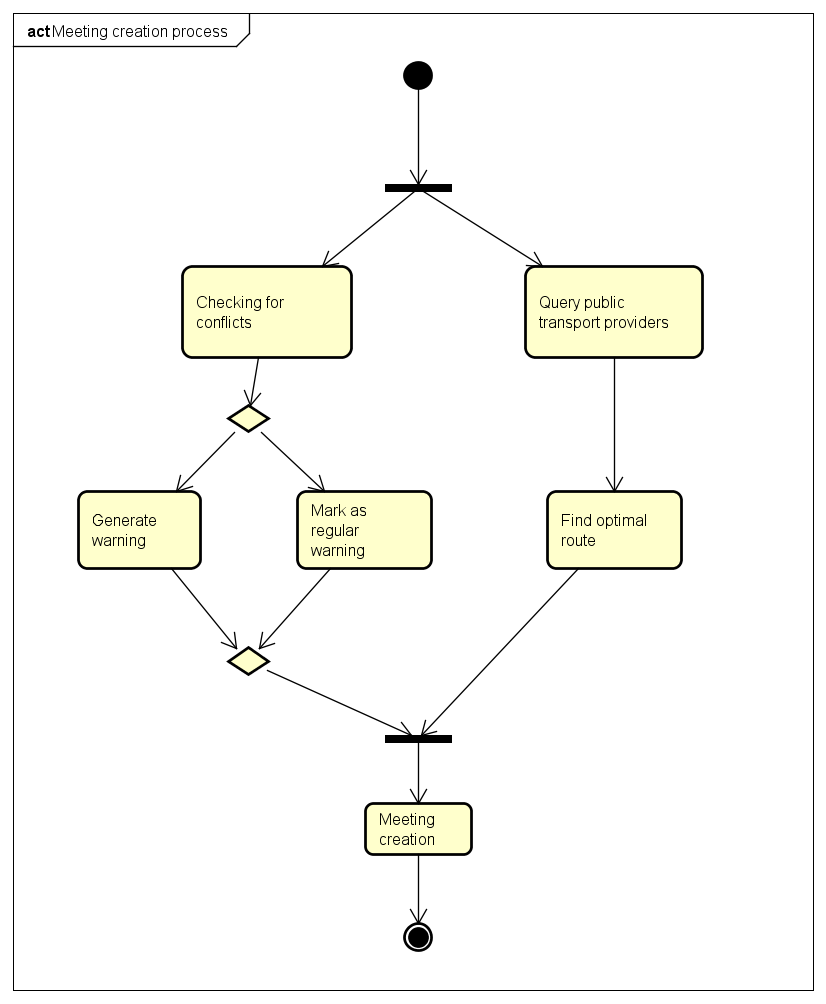
\includegraphics[width=\textwidth]{activitydiagrams/meetingcreationprocess} 
\caption{This diagram shows the activities carried out by the system in the meeting creation process} 
\label{fig:meetingcreationprocess} 
\end{figure} 
